%!TEX program = xelatex
% 完整编译: xelatex -> biber/bibtex -> xelatex -> xelatex
\documentclass[lang=cn,a4paper]{elegantpaper}

\title{ElegantPaper: 一个优美的 \LaTeX{} 工作论文模板}
\author{Ethan DENG \\ Fudan University \and Dongsheng DENG \\ PA Technology}
\institute{\href{https://elegantlatex.org/}{Elegant\LaTeX{} 项目组}}

\version{0.10}
\date{\zhtoday}


% 本文档命令
\usepackage{makecell}
\usepackage{array}
\usepackage{graphicx}
\usepackage[rightcaption]{sidecap}
\newcommand{\ccr}[1]{\makecell{{\color{#1}\rule{1cm}{1cm}}}}
\addbibresource[location=local]{reference.bib} % 参考文献,不要删除

\begin{document}

\maketitle

\begin{abstract}
本文为 \href{https://github.com/ElegantLaTeX/ElegantPaper/}{ElegantPaper} 的说明文档。此模板基于 \LaTeX{} 的 article 类,专为工作论文写作而设计。设计这个模板的初衷是让作者不用关心工作论文的格式,专心写作,从而有更加舒心的写作体验。如果你有其他问题、建议或者报告 bug,可以在 \href{https://github.com/ElegantLaTeX/ElegantPaper/issues}{GitHub::ElegantPaper/issues} 留言。如果你想了解更多 Elegant\LaTeX{} 项目组设计的模板,请访问 \href{https://github.com/ElegantLaTeX/}{GitHub::ElegantLaTeX}。
\keywords{Elegant\LaTeX{},工作论文,模板}
\end{abstract}

\section{问题定义}

\subsection{项目背景及意义}

\subsubsection{项目背景}

如今Linux系统被广泛使用,我们需要一种中心化的机制用于搜索以及安装软件。然而软件通常需要存放在存储库里,
并通过包的形式进行分发。我们需要一个方便好用的包管理系统来安装更新包文件,同时确定包中的代码是经过审核以
及得到过开发人员以及包维护人员的认可。当然我们也可以通过一些现有的开发好的软件商店进行软件的安装,他们的优势是
具有一个图形化的界面,可以使用鼠标点击安装,在使用上更加人性化,现有的应用商店有 GNOME Software, Discover, 
AppCenter等,虽然他们都已经有了十分成熟的系统机制,但是依然或多或少的缺点,例如他们大部分之运行都有一定的限制,
例如GNOME Software和Discover和桌面环境深度绑定,因此我们决定开发一款基于electron的跨发行版跨桌面的的应用商店,
为用户提供更加美观,人性化的界面\ref{UnixAppstore}。

\begin{figure}[ht]
    \centering
    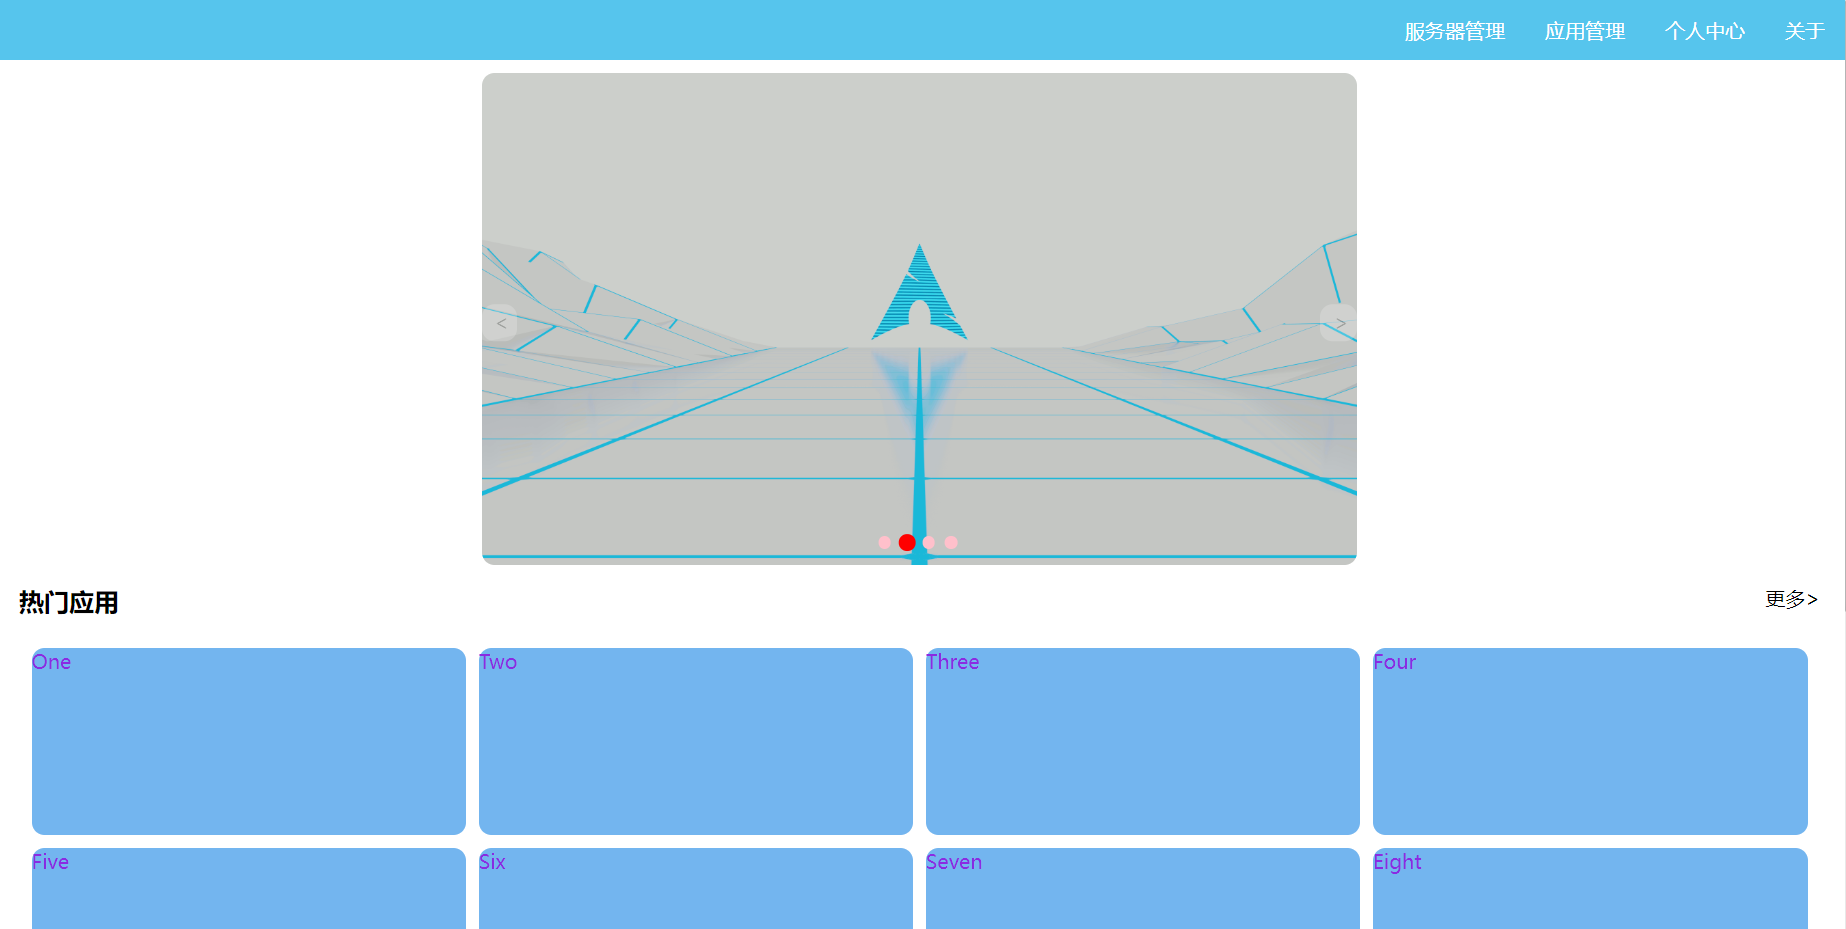
\includegraphics[scale=0.25]{./image/UnixAppstore}
    \caption{UnixAppstore}
	\label{UnixAppstore}
\end{figure}

\subsubsection{项目意义}

为什么开发这款应用呢?我们这款应用的开发能给广大的Linux用户带来更加舒适的体验,同时大家也能够更好的接触新的软件包,除此之外我们会及时更新软件包,不像其他部分软件商店可能会存在部分软件包过时,而我们这款应用商店不会存在软件包过时的情况。这个世界每一分钟都有上千种技术被发明,而我们这一款应用也会及时推送一些新产生的软件包,这样就可以及时让你接触到这些新奇的事物,或许你也能从中找到灵感,进而进行二次开发。

与此同时我们能为用户提供一个更美观,人性化的界面以及使其远端同步服务器的数据,并且针对开发者我们这款应用能够是他们获取资源进行二次开发,并且发布自己的软件包并且进行管理。

\subsection{项目基本目标}
本项目致力于开发一款跨平台的应用,在不同的Linux发行版本都可以进行软件包的下载与安装,我们将通过ArcLinux的API对AUR中的软件包进行查询,获取相应的资源文件并存储于本地,然后通过与自己的Linux服务器进行ssh连接,进而传递到自己的服务器上。这也是跨平台实现的核心,当然可以连接同时连接不同的服务器,这也表明可以同时与多台服务器进行交互。同时我们希望能够在应用中开发一个webshell界面,方便使用指令进行交互。

当前我们处于ssh连接服务器阶段,我们需要利用ip地址,host用户名进行远程服务器的连接,同时我们需要实现开发者上传软件包功能包到远端服务器,这样也就为大家获取更新的软件包提供了来源。

下一步我们将进行应用的后端开发,我们需要处理开发者上传的软件包以及加合适可靠的软件包加载到搜索的源中,这样用户就可以通过应用搜索获取相应的软件包,更后面我们将会将会进行服务器端的开发,将登陆注册逻辑以及软件包下载安装逻辑放在服务器端,这样能够进一步的提升软件的运行速度。

最终目标当然是实现一个功能完善,用户体验良好的跨平台桌面软件商店,这要求我们软件的可用性,可靠性,可移植性良好并且拥有美观的UI界面如图\ref{UnixAppstore}。


\subsection{可行性分析}

如今市面上比较流行的有基于GNOME的GNOME Software如图\ref{UbuntuSoftware} 以及基于KDE的 DisCover如图\ref{KDEDiscover}, AppCenter等等,它们都发展的相对成熟,但是他们都有自己的弊端,基本上都需要相关的桌面环境的支持,这就导致不能单单只下载应用,你需要下载安装配套的桌面环境,除此之外像AppCenter就是只提供对Ubuntu存储库的访问。综上我们能看出,对于一个跨平台的应用商店是很有市场的,也是广大用户所希望的,除此之外,针对用户来说,更快的接触到有保障的新软件包,新技术也是其的需求之一。

现有的软件商店各有其优缺点,如GNOME Software,其虽然拥有较多的软件包资源,但是UI界面并不美观如图\ref{KDEDiscover},以及其存在部分软件包严重的过时导致不可用,又如KDE Discover,其官方虽然会进场收录一些社区软件进入其应用商店,但是总体来说数量还是相对较少,而我们所开发的UnixAppstore不仅会提供一个美观吸引人的UI界面如图\ref{UnixAppstore},还会提供大量的软件资源,以及我们会及时的更新软件资源,这也是我们优势之一。

\begin{figure}[ht]
    \centering
    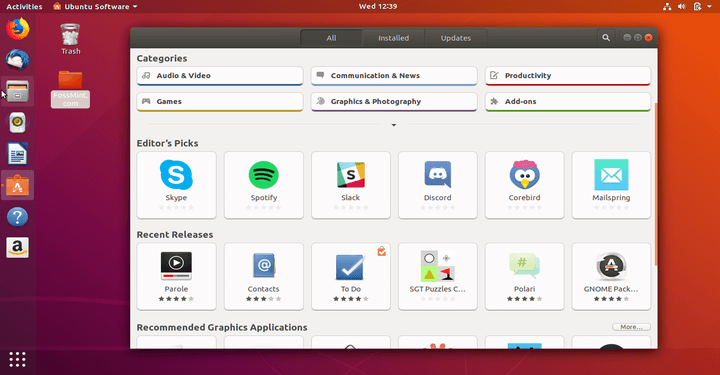
\includegraphics[scale=0.5]{./image/UbuntuSoftware}
    \caption{Ubuntu-Software}
	\label{UbuntuSoftware}
\end{figure}

\begin{figure}[ht]
    \centering
    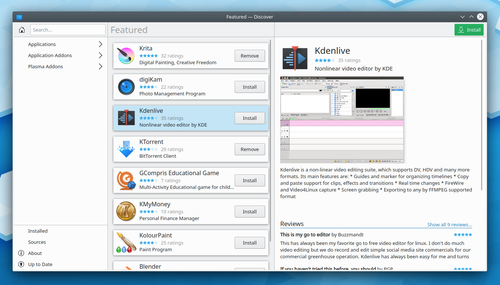
\includegraphics[scale=0.96]{./image/KDEDiscover}
    \caption{KDE-Discover}
	\label{KDEDiscover}
\end{figure}


为什么这款软件是可以实现跨平台的呢?这是因为我们是基于electron这个桌面框架进行开发,而由架构于electron开发的VSCode已经很好的证明electron这个框架实现跨平台应用并且能够做的很好,这也是我们信心的来源。但是当前实现技术方面我们需要实现用户远程连接服务器,进而将软件资源传递给远端服务器,同时我们也需要支持用户直接操作远端服务器,除此之外我们需要将获取的软件包进行解析到本地,以及对于开发者上传到软件包到服务器,我们需要将软件包进行可靠性分析测试,并在测试完成后将其上传到我们的软件搜索源中。

技术上,上述问题都是可实现的,首先在连接远端服务器我们可以通过ssh技术进行连接,用户上传文件至远端服务器我们可以通过post进行操作,除此之外我们会开发一个webshell界面方便用户对远端服务器进行指令交互,针对开发者上传软件包我们需要判断其来源是否可靠,以及其中是否包含病毒,在测试完成后我们再进一步将其上传至服务器并同步更新搜索源内容。

由于同类型的应用商店较少,所以市场的竞争压力相对较少,并且留给我们的市场相对广阔,市场前景非常良好。


\subsection{人员管理和项目进度管理}

我们项目组只有两个成员,目前程家骏负责软件源的解析以及开发者界面的设计,刘俊潇负责远端服务器的连接,登陆注册界面的设计,以及后续webshell的开发设计。在完成当前任务后,程家骏将负责服务器端的开发,刘俊潇将负责前端方面的开发。

项目进度的管理

\begin{tabular}{|l|c|c|}%一个c表示有一列,格式为居中显示(center)
\hline
日期&程家骏&刘俊潇\\
\hline
2022/9/23 - 2022/9/30&实现软件的主界面以及个人主页&实现登陆注册界面\\%第二行第一列和第二列  中间用&连接
\hline
2022/9/31 - 2022/10/5&获取软件包资源并进行解析&开发AUR界面并且实现用户免密登陆 \\
\hline
2022/10/6 - 2022/10/20&\makecell[c]{实现搜索功能,并且对服务器界面\\以及开发者界面进行开发}&\makecell[c]{完成about界面\\以及部分server界面的开发}\\
\hline
\end{tabular}

\subsubsection{方正字体选项}
由于使用 \lstinline{ctex} 宏包默认调用系统已有的字体,部分系统字体缺失严重,因此,用户希望能够使用其它字体,我们推荐使用方正字体。方正的{\songti 方正书宋}、{\heiti 方正黑体}、{\kaishu 方正楷体}、{\fangsong 方正仿宋}四款字体均可免费试用,且可用于商业用途。用户可以自行从\href{http://www.foundertype.com/}{方正字体官网}下载此四款字体,在下载的时候请\textbf{务必}注意选择 GBK 字符集,也可以使用 \href{https://www.latexstudio.net/}{\LaTeX{} 工作室}提供的\href{https://pan.baidu.com/s/1BgbQM7LoinY7m8yeP25Y7Q}{方正字体,提取码为:njy9} 进行安装。安装时,{\kaishu Win 10 用户请右键选择为全部用户安装,否则会找不到字体。}

\begin{figure}[!htb]
\centering
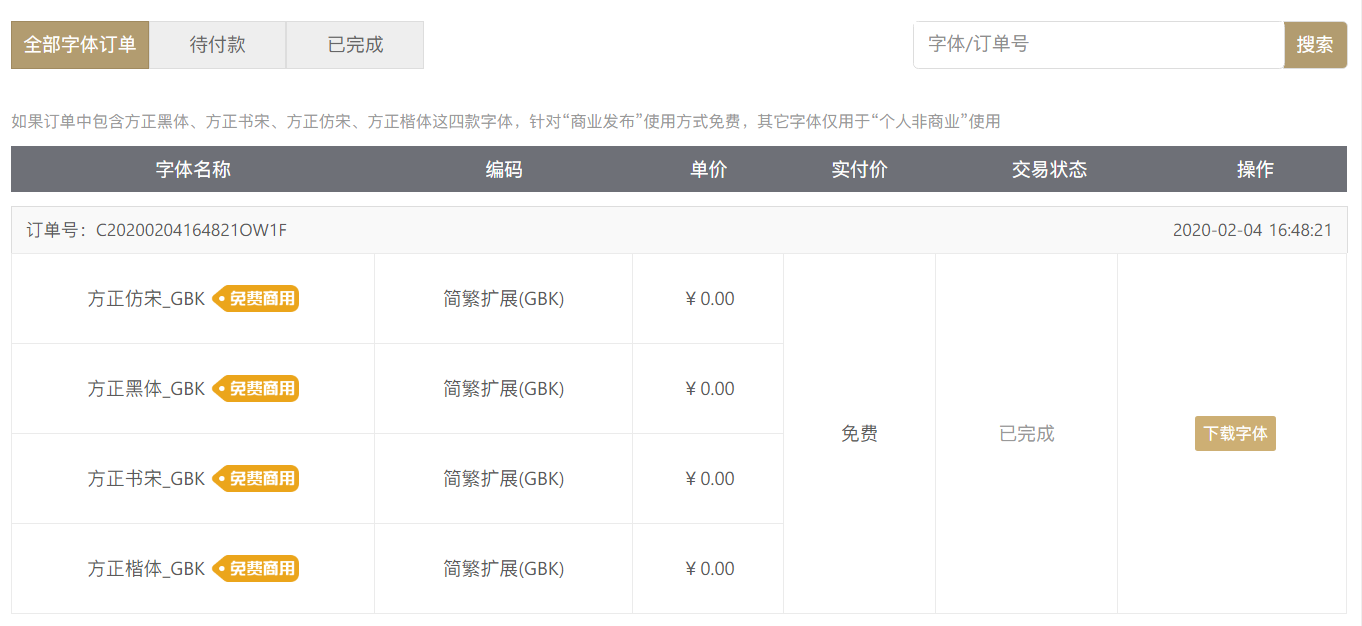
\includegraphics[width=0.9\textwidth]{founder.png}
\end{figure}

\subsubsection{其他中文字体}
如果你想完全自定义字体\footnote{这里仍然以方正字体为例。},你可以选择 \lstinline{chinesefont=nofont},然后在导言区设置即可,可以参考下方代码:
\begin{lstlisting}
\setCJKmainfont[BoldFont={FZHei-B01},ItalicFont={FZKai-Z03}]{FZShuSong-Z01}
\setCJKsansfont[BoldFont={FZHei-B01}]{FZKai-Z03}
\setCJKmonofont[BoldFont={FZHei-B01}]{FZFangSong-Z02}
\setCJKfamilyfont{zhsong}{FZShuSong-Z01}
\setCJKfamilyfont{zhhei}{FZHei-B01}
\setCJKfamilyfont{zhkai}[BoldFont={FZHei-B01}]{FZKai-Z03}
\setCJKfamilyfont{zhfs}[BoldFont={FZHei-B01}]{FZFangSong-Z02}
\newcommand*{\songti}{\CJKfamily{zhsong}}
\newcommand*{\heiti}{\CJKfamily{zhhei}}
\newcommand*{\kaishu}{\CJKfamily{zhkai}}
\newcommand*{\fangsong}{\CJKfamily{zhfs}}
\end{lstlisting}



\subsection{自定义命令}
此模板并没有修改任何默认的 \LaTeX{} 命令或者环境\footnote{目的是保证代码的可复用性,请用户关注内容,不要太在意格式,这才是本工作论文模板的意义。}。另外,我自定义了 4 个命令:
\begin{enumerate}
  \item \lstinline{\email}:创建邮箱地址的链接,比如 \email{ddswhu@outlook.com};
  \item \lstinline{\figref}:用法和 \lstinline{\ref} 类似,但是会在插图的标题前添加 <\textbf{图 n}> ;
  \item \lstinline{\tabref}:用法和 \lstinline{\ref} 类似,但是会在表格的标题前添加 <\textbf{表 n}>;
  \item \lstinline{\keywords}:为摘要环境添加关键词。
\end{enumerate}

\subsection{参考文献}

文献部分,本模板调用了 biblatex 宏包,并提供了 biber(默认) 和 bibtex 两个后端选项,可以使用 \lstinline{bibend} 进行修改:

\begin{lstlisting}
  \documentclass[bibtex]{elegantpaper}
  \documentclass[bibend=bibtex]{elegantpaper}
\end{lstlisting}

关于文献条目(bib item),你可以在谷歌学术,Mendeley,Endnote 中取,然后把它们添加到 \lstinline{reference.bib} 中。在文中引用的时候,引用它们的键值(bib key)即可。

为了方便文献样式修改,模板引入了 \lstinline{bibstyle} 和 \lstinline{citestyle} 选项,默认均为数字格式(numeric),参考文献示例:\cite{cn1,en2,en3} 使用了中国一个大型的 P2P 平台(人人贷)的数据来检验男性投资者和女性投资者在投资表现上是否有显著差异。

如果需要设置为国标 GB7714-2015,需要使用:
\begin{lstlisting}
  \documentclass[citestyle=gb7714-2015, bibstyle=gb7714-2015]{elegantpaper} 
\end{lstlisting}

如果需要添加排序方式,可以在导言区加入
\begin{lstlisting}
  \ExecuteBibliographyOptions{sorting=ynt}
\end{lstlisting}

启用国标之后,可以加入 \lstinline{sorting=gb7714-2015}。


\section{使用 newtx 系列字体}

如果需要使用原先版本的 \lstinline{newtx} 系列字体,可以通过显示声明数学字体:

\begin{lstlisting}
\documentclass[math=newtx]{elegantpaper}
\end{lstlisting}

\subsection{连字符}

如果使用 \lstinline{newtx} 系列字体宏包,需要注意下连字符的问题。
\begin{equation}
  \int_{R^q} f(x,y) dy.\emph{of\kern0pt f}
\end{equation}

\begin{lstlisting}
\begin{equation}
  \int_{R^q} f(x,y) dy.\emph{of \kern0pt f}
\end{equation}
\end{lstlisting}

\subsection{宏包冲突}

有用户反馈模板在使用 \lstinline{yhmath} 以及 \lstinline{esvect} 等宏包时会报错:
\begin{lstlisting}
LaTeX Error:
   Too many symbol fonts declared.
\end{lstlisting}

原因是在使用 \lstinline{newtxmath} 宏包时,重新定义了数学字体用于大型操作符,达到了 {\heiti 最多 16 个数学字体} 的上限,在调用其他宏包的时候,无法新增数学字体。为了减少调用非常用宏包,在此给出如何调用 \lstinline{yhmath} 以及 \lstinline{esvect} 宏包的方法。

请在 \lstinline{elegantpaper.cls} 内搜索 \lstinline{yhmath} 或者 \lstinline{esvect},将你所需要的宏包加载语句\textit{取消注释}即可。


\section{常见问题 FAQ}

\begin{enumerate}[label=\arabic*).]
  \item \textit{如何删除版本信息?}\\
    导言区不写 \lstinline|\version{x.xx}| 即可。
  \item \textit{如何删除日期?}\\
    需要注意的是,与版本 \lstinline{\version} 不同的是,导言区不写或注释 \lstinline{\date} 的话,仍然会打印出当日日期,原因是 \lstinline{\date} 有默认参数。如果不需要日期的话,日期可以留空即可,也即 \lstinline|\date{}|。
  \item \textit{如何获得中文日期?}\\
    为了获得中文日期,必须在中文模式下\footnote{英文模式下,由于未加载中文宏包,无法输入中文。},使用 \lstinline|\date{\zhdate{2019/10/11}}|,如果需要当天的汉化日期,可以使用 \lstinline|\date{\zhtoday}|,这两个命令都来源于 \href{https://ctan.org/pkg/zhnumber}{\lstinline{zhnumber}} 宏包。
  \item \textit{如何添加多个作者?}\\
    在 \lstinline{\author} 里面使用 \lstinline{\and},作者单位可以用 \lstinline{\\} 换行。
    \begin{lstlisting}
    \author{author 1\\ org. 1 \and author 2 \\ org. 2 }
    \end{lstlisting}
  \item \textit{如何添加中英文摘要?}\\
    请参考 \href{https://github.com/ElegantLaTeX/ElegantPaper/issues/5}{GitHub::ElegantPaper/issues/5}
\end{enumerate}


\section{致谢}

特别感谢 \href{https://github.com/sikouhjw}{sikouhjw} 和 \href{https://github.com/syvshc}{syvshc}  长期以来对于 Github 上 issue 的快速回应,以及各个社区论坛对于 ElegantLaTeX 相关问题的回复。特别感谢 ChinaTeX 以及 \href{http://www.latexstudio.net/}{LaTeX 工作室} 对于本系列模板的大力宣传与推广。

如果你喜欢我们的模板,你可以在 Github 上收藏我们的模板。

\nocite{*}
\printbibliography[heading=bibintoc, title=\ebibname]

\appendix
%\appendixpage
\addappheadtotoc

\end{document}
